\documentclass[11pt,a4paper]{article}
\usepackage[margin=2.3cm]{geometry}
\usepackage[T1]{fontenc}
\usepackage{lmodern}
\usepackage{microtype}
\usepackage{booktabs}
\usepackage{graphicx}
\usepackage{float}
\usepackage{caption}
\usepackage[numbers]{natbib}
\usepackage[hidelinks]{hyperref}
\usepackage{xcolor}

\setlength{\parskip}{0.5em}
\setlength{\parindent}{0pt}
\captionsetup{font=small,labelfont=bf}
\graphicspath{{figures/}}

% Every number below is generated from MLflow and the data by scripts/make_report_assets.py.
% Generated by scripts/make_report_assets.py - do not edit.
\newcommand{\AblAddDayOfWeek}{3.00}
\newcommand{\AblNoDistanceXMarket}{0.28}
\newcommand{\AblNoLabelScreen}{14.18}
\newcommand{\AblNoMarket}{34.11}
\newcommand{\AblNoQuarterEnd}{28.99}
\newcommand{\AblNoTrend}{13.34}
\newcommand{\AblResidualTreesWithoutMarket}{0.86}
\newcommand{\CappedWeights}{1,204}
\newcommand{\ChampionRun}{f51bb0ec64524e3eb1d170f3ee1765a4}
\newcommand{\CorruptPct}{1.41}
\newcommand{\CorruptRows}{677}
\newcommand{\CorruptShareOfError}{59}
\newcommand{\CoverEighty}{84.7}
\newcommand{\CoverEightyAll}{83.5}
\newcommand{\CoverNinetyFive}{96.9}
\newcommand{\CoverNinetyFiveAll}{95.5}
\newcommand{\DecFirst}{829.08}
\newcommand{\DecFlatMax}{863.82}
\newcommand{\DecFlatMin}{838.79}
\newcommand{\DecLast}{877.62}
\newcommand{\DecLastNoRamp}{857.83}
\newcommand{\DecMax}{877.62}
\newcommand{\DecMin}{829.08}
\newcommand{\DevNaiveIndex}{74.61}
\newcommand{\DevStepA}{157.55}
\newcommand{\DevStepB}{111.25}
\newcommand{\DevStepC}{63.77}
\newcommand{\DevStepD}{44.01}
\newcommand{\DevStepE}{42.67}
\newcommand{\DevStepF}{42.30}
\newcommand{\DevTunedGain}{0.36}
\newcommand{\DevTunedGainHigh}{0.45}
\newcommand{\DevTunedGainLow}{0.30}
\newcommand{\DistanceMarket}{0.015}
\newcommand{\DriftPerMonth}{0.62}
\newcommand{\ElasticityDay}{0.154}
\newcommand{\ElasticityLoad}{0.127}
\newcommand{\FitSeconds}{1.8}
\newcommand{\HiddenCitiesPerFold}{8}
\newcommand{\HorizonDays}{61}
\newcommand{\InferenceMicroseconds}{46}
\newcommand{\LaredoDegreesSouth}{2.9}
\newcommand{\LockedTestRun}{95fb9814916747019528b05e5b28c031}
\newcommand{\MapeDevStepA}{8.56}
\newcommand{\MapeDevStepB}{5.74}
\newcommand{\MapeDevStepC}{2.71}
\newcommand{\MapeDevStepD}{1.84}
\newcommand{\MapeDevStepE}{1.79}
\newcommand{\MapeDevStepF}{1.78}
\newcommand{\MapeTestFinal}{1.56}
\newcommand{\MarketBetweenDaySD}{0.167}
\newcommand{\MarketWithinDaySD}{0.025}
\newcommand{\MissingMarket}{374}
\newcommand{\MissingWeights}{300}
\newcommand{\NTrain}{48,000}
\newcommand{\NValidation}{12,000}
\newcommand{\NegativeWeights}{292}
\newcommand{\NestedGainFive}{0.48}
\newcommand{\NestedGainFour}{0.50}
\newcommand{\NestedRun}{e5ab30f226be}
\newcommand{\OctoberUnderForecast}{1.1}
\newcommand{\QuoteCopyMax}{0.99}
\newcommand{\QuoteCopyMin}{0.88}
\newcommand{\QuoteDistanceCorrTrain}{0.81}
\newcommand{\QuoteDistanceCorrValidation}{0.01}
\newcommand{\QuoteMirrorMax}{-0.94}
\newcommand{\QuoteMirrorMin}{-0.82}
\newcommand{\RampDryVan}{2.3}
\newcommand{\RampFlatbed}{7.8}
\newcommand{\RampReefer}{5.0}
\newcommand{\RecencyTau}{122.6}
\newcommand{\RidgeAlpha}{0.265}
\newcommand{\RmseTestMax}{669}
\newcommand{\RmseTestMin}{630}
\newcommand{\RowsAfterScreen}{47,323}
\newcommand{\ScreenHigh}{1.5}
\newcommand{\ScreenLow}{0.67}
\newcommand{\SeenWeight}{87.94}
\newcommand{\TestBaselineLaneRatePerMile}{90.66}
\newcommand{\TestBaselineNaiveIndex}{73.98}
\newcommand{\TestCatboostRawDollars}{64.31}
\newcommand{\TestEquipmentRatePerMile}{175.52}
\newcommand{\TestFinalAllMAE}{91.86}
\newcommand{\TestFinalTuned}{38.14}
\newcommand{\TestGapBaselineLaneRatePerMile}{50.75}
\newcommand{\TestGapBaselineLaneRatePerMileHigh}{56.29}
\newcommand{\TestGapBaselineLaneRatePerMileLow}{46.00}
\newcommand{\TestGapBaselineNaiveIndex}{35.45}
\newcommand{\TestGapBaselineNaiveIndexHigh}{44.51}
\newcommand{\TestGapBaselineNaiveIndexLow}{28.68}
\newcommand{\TestGapCatboostRawDollars}{27.35}
\newcommand{\TestGapCatboostRawDollarsHigh}{32.21}
\newcommand{\TestGapCatboostRawDollarsLow}{22.60}
\newcommand{\TestGapEquipmentRatePerMile}{136.88}
\newcommand{\TestGapEquipmentRatePerMileHigh}{143.86}
\newcommand{\TestGapEquipmentRatePerMileLow}{131.58}
\newcommand{\TestGapLightgbmLogMarketCalendar}{11.30}
\newcommand{\TestGapLightgbmLogMarketCalendarHigh}{14.42}
\newcommand{\TestGapLightgbmLogMarketCalendarLow}{8.01}
\newcommand{\TestGapRidgePlusResidualTrees}{-0.42}
\newcommand{\TestGapRidgePlusResidualTreesHigh}{-0.05}
\newcommand{\TestGapRidgePlusResidualTreesLow}{-0.81}
\newcommand{\TestGapStructuralRidge}{1.04}
\newcommand{\TestGapStructuralRidgeHigh}{2.08}
\newcommand{\TestGapStructuralRidgeLow}{0.15}
\newcommand{\TestLightgbmLogMarketCalendar}{48.94}
\newcommand{\TestRidgePlusResidualTrees}{37.88}
\newcommand{\TestStructuralRidge}{39.40}
\newcommand{\TuneBest}{42.30}
\newcommand{\TuneMatchesFinal}{yes}
\newcommand{\TuneTrials}{60}
\newcommand{\TunedDefaultTestPct}{1.1}
\newcommand{\TuningRun}{dee389aba0bd}
\newcommand{\UnseenCities}{8}
\newcommand{\UnseenCityList}{Allentown, Charlotte, Chicago, Jackson, Knoxville, Laredo, Norfolk, San Diego}
\newcommand{\UnseenShare}{12.06}
\newcommand{\UnseenWeight}{12.06}

\newcommand{\usd}[1]{\$#1}
\newcommand{\inputtable}[1]{\begin{center}\small\resizebox{\ifdim\width>\linewidth\linewidth\else\width\fi}{!}{\input{tables/#1.tex}}\end{center}}

\title{Freight Rate Prediction\\[0.3em]\large Data, validation, model and results}
\author{Hasin Ahmed}
\date{October 2026}

\begin{document}
\maketitle
\tableofcontents
\clearpage

\section{Summary}

\textbf{The task.} We predict the posted rate, in dollars, for \NValidation{} truckload shipments (``loads'') moving
in November and December 2025. We learn from \NTrain{} labelled loads from January to October 2025. We also draw a
daily December forecast for one fixed lane.

\textbf{Why it is hard.} The scoring months come after every training month, so this is a forecast, not an
interpolation. About \CorruptPct\% of the training rates are recording errors. \UnseenShare\% of the scoring loads
touch cities that never appear in training.

\textbf{The model.} A two-stage model. Stage one is a ridge regression\footnote{Linear regression with a small
penalty on large coefficients, which keeps estimates stable \citep{hoerl1970ridge}.} on the logarithm of the rate.
It describes the load (distance, weight, location, equipment) and the market (the daily market index, a slow upward
drift and a price ramp near quarter ends). Stage two is a small LightGBM tree ensemble \citep{ke2017lightgbm} that
corrects what stage one leaves over. Recent loads count more than old ones in training.

\textbf{Headline numbers.} We measure error as the mean absolute error in dollars on loads with plausible labels,
re-weighted to the scoring mix of new and known cities (``wMAE'', Section~\ref{sec:validation}).
\begin{itemize}
  \item Development folds: \usd{\DevStepF} (\MapeDevStepF\% of the rate), against \usd{\DevStepA} for the simplest
        sensible price and \usd{\DevStepB} for the original CatBoost submission.
  \item Locked test (September--October 2025, evaluated once): \usd{\TestFinalTuned} (\MapeTestFinal\%), against
        \usd{\TestCatboostRawDollars} for the original submission.
  \item December 31 chart value: \usd{\DecLast}.
\end{itemize}

\textbf{Main caveats.} Tuning bought \usd{\DevTunedGain} on the development folds, but on the locked test the
untuned version was slightly better; the two are practically equivalent. The test period had already been
inspected by earlier work, so its numbers are mildly optimistic. December relies on the quarter-end ramp recurring.

\section{Problem and data}

\textbf{Files.} Four CSV files define the task.
\begin{itemize}
  \item \texttt{train-test.csv}: \NTrain{} loads from 1 January to 31 October 2025, with the posted rate.
  \item \texttt{validation.csv}: \NValidation{} loads from 1 November to 31 December 2025, without rates. These are
        the loads we must price.
  \item \texttt{validation-predictions-template.csv}: the load IDs, in the order the submission must follow.
  \item \texttt{december-chart-inputs.csv}: one load (Lexington to Fort Wayne, 360 miles, Dry Van, 32,000 lb)
        for every day of December.
\end{itemize}

\textbf{Columns.} Each load has a pickup and delivery city with coordinates, the road distance, the equipment type
(Dry Van, Reefer or Flatbed), the weight, the date, a \texttt{market\_index} and a \texttt{quote\_signal}.

\textbf{Target.} The posted rate in dollars. We model its logarithm, so errors are relative and a 2\% miss counts
the same on a \usd{300} and a \usd{5,000} load. The forecast is the exponential of the predicted logarithm, which
estimates the median rate.

\textbf{Horizon.} On 31 October we know every label so far and must price loads 1 to 61 days ahead.
The market index of each target day is known, because it is a column of the scoring file.

\textbf{Unseen cities.} \UnseenCities{} cities in the scoring file never appear in training (\UnseenCityList).
They touch \UnseenShare\% of the scoring loads. A model that memorises city names cannot price them, so the model
uses coordinates instead.

\textbf{Metric.} The assessment does not name a scoring metric. We chose the mean absolute error in dollars
(Section~\ref{sec:validation}) and report several others next to it.

\section{Data quality and preprocessing}

All fixes in this section use only the load's own columns or other loads on the same date. None reads the rate, so
they can run before any split without leaking information.

\textbf{Corrupted labels.} For each load we compare its rate per mile with the median of its lane and equipment.
Clean loads sit in a narrow peak. \CorruptRows{} loads (\CorruptPct\%) sit in two separate bands, at about 0.2--0.5
and 2--5 times the lane norm, with almost nothing in between (Figure~\ref{fig:noise}). They appear at the same rate
in every month and equipment type, and no feature predicts them. We treat them as recording errors.

\begin{figure}[H]
  \centering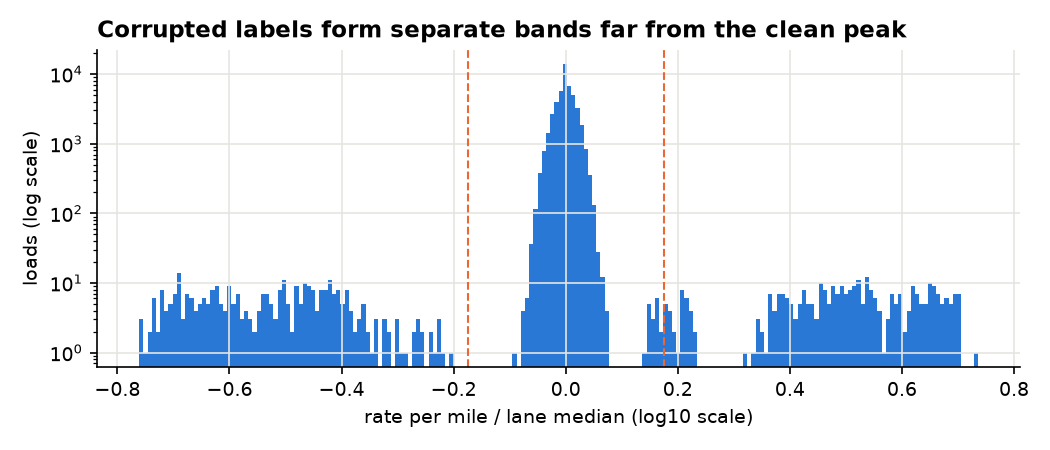
\includegraphics[width=0.8\linewidth]{label_noise.png}
  \caption{Rate per mile relative to the lane median. Dashed lines: the \ScreenLow{} and \ScreenHigh{} screening bounds.}
  \label{fig:noise}
\end{figure}

\emph{Treatment.} Inside every training fold a robust two-pass ridge fit flags rows outside \ScreenLow--\ScreenHigh{} times its
prediction, and those rows are left out of training. The screen is learned, so it never sees assessment rows.
For reporting we use a separate fixed flag (the lane-median ratio above). It marks the same kind of row for every
model and is never used in fitting. Removing the screen costs \usd{\AblNoLabelScreen} on the development folds
(Section~\ref{sec:features}).

\textbf{Negative weights.} \NegativeWeights{} training loads have negative weights whose sizes match normal
weights. These are sign-entry errors, so we use the absolute value.

\textbf{Weight cap.} \CappedWeights{} loads sit exactly at 47,500 lb, a ceiling. A flag tells the model a weight
is capped.

\textbf{Missing values.} \MissingWeights{} weights are missing; we fill them with 31,000 lb (about the median), and
the tree stage sees them as missing. \MissingMarket{} market-index readings are missing; we fill each with that
day's mean, because readings vary little within a day (standard deviation \MarketWithinDaySD) compared with between
days (\MarketBetweenDaySD).

\textbf{Why quote\_signal is dropped.} In training months, \texttt{quote\_signal} either copies the rate per mile
(correlation \QuoteCopyMin{} to \QuoteCopyMax) or mirrors it (\QuoteMirrorMin{} to \QuoteMirrorMax), depending on
the month (Figure~\ref{fig:quote}). In the scoring months that relationship is gone: its correlation with log
distance is \QuoteDistanceCorrValidation, against a typical \QuoteDistanceCorrTrain{} in training. A model that
used it would learn a leak that does not exist when predictions are made. It is never a model input, and a unit
test checks that predictions do not change when it is replaced by noise. Load IDs and city names are not inputs
either.

\begin{figure}[H]
  \centering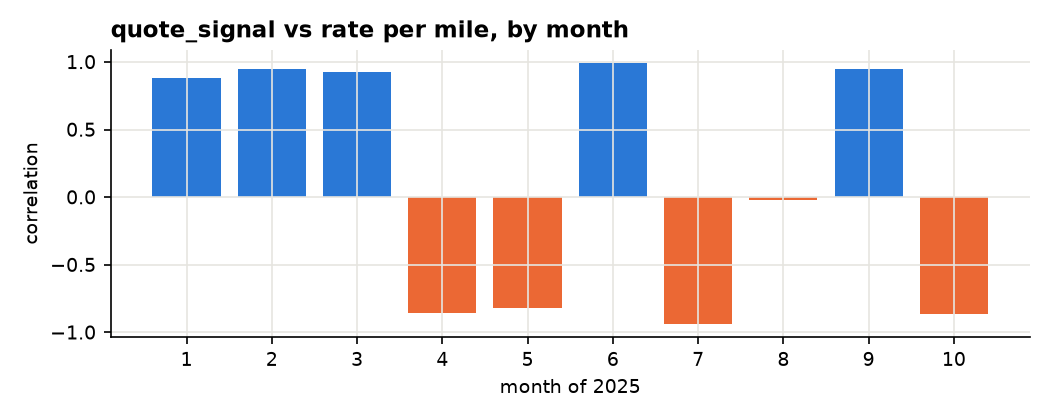
\includegraphics[width=0.8\linewidth]{quote_signal.png}
  \caption{Monthly correlation of \texttt{quote\_signal} with the rate per mile (clean training rows).}
  \label{fig:quote}
\end{figure}

\section{Validation design}\label{sec:validation}

\textbf{Rolling-origin folds.} A fold mimics the real situation once. We pick a cut-off date (the ``origin''),
train on every load up to it, and score the loads of the next \HorizonDays{} days. We use five origins: the last day of
February, March, April, May and June 2025. Each fold's training window grows with time (``expanding window'').
This is the standard way to evaluate forecasts \citep{hyndman2021fpp3}. A random split would mix future and past
loads and reward features that only work by looking ahead.

\textbf{Hidden cities.} In every fold, \HiddenCitiesPerFold{} random cities (fixed seed: 100 plus the fold number) are removed from
training. Their loads still appear in the scored period. This mimics the \UnseenShare\% of scoring loads that touch
new cities.

\textbf{Locked test.} The last origin, 31 August, scores September and October. Nothing about the model was chosen
on it. It was evaluated once, after the final configuration was frozen, by a script that refuses to run twice.
One honest caveat: earlier analyses of this project had already looked at these months, so the test is not fully
untouched. No untouched labelled period exists.

\textbf{Metric.} We report the mean absolute error (MAE) in dollars on loads with plausible labels. Loads touching
hidden cities and other loads are re-weighted to the scoring mix (\UnseenWeight\% and \SeenWeight\%). We call this
\emph{wMAE}. We chose it for three reasons.
\begin{itemize}
  \item It is in dollars, the unit of the business question.
  \item It is robust to the corrupted labels. On the locked test those \CorruptPct\% of loads produce
        \CorruptShareOfError\% of all absolute error.
  \item It matches the median forecast that the log model produces.
\end{itemize}
The root mean squared error (RMSE) squares each error, so a handful of 3-to-5-times label errors dominate it. On the test period
every model in this report scores an RMSE between \usd{\RmseTestMin} and \usd{\RmseTestMax}, whatever its quality, so
RMSE cannot rank models here. We still report it, together with MAPE (mean absolute percentage error) and bias.

\textbf{Comparing two models.} Differences come with a 95\% interval from a paired block bootstrap. Both models are
scored on the same loads; we resample whole 7-day blocks of days, because loads on nearby days share the market
and are not independent \citep{kunsch1989jackknife}.

\section{Feature engineering}\label{sec:features}

Each feature below has a plain definition, the reason it should help, and the result of removing it (or adding it)
on the five development folds. The removals are made one at a time on the untuned ridge-plus-trees model (ladder
step 5, \usd{\DevStepE}), following the advice to test feature groups against out-of-sample error rather than
importance scores \citep{kuhn2019feature}. Table~\ref{tab:ablations} has every result with its paired interval.

\begin{description}
  \item[Load description.] Smooth curves (cubic B-splines) of log distance, weight and the four pickup and delivery
    coordinates, a weight-at-cap flag, and equipment dummies with Dry Van as the reference. Price per mile falls
    smoothly with distance and varies smoothly with location. Coordinates, unlike city names, also work for cities
    the model has never seen.
  \item[market\_level\_today.] The logarithm of the day's mean market index. Its coefficient is an elasticity: the
    fitted model moves the rate by \ElasticityDay\% for each 1\% change in the day's index. Removing the market
    costs \usd{\AblNoMarket}, the largest single loss.
  \item[market\_deviation\_this\_load.] The load's own log index minus the day's mean (elasticity \ElasticityLoad).
  \item[days\_since\_start.] A linear drift beyond the market, \DriftPerMonth\% per month in the final model.
    Removing it costs \usd{\AblNoTrend}; without it every later window is under-forecast.
  \item[quarter\_end\_progress $\times$ equipment.] Zero on the 1st and one on the last day of March, June,
    September and December; zero in other months. Prices ramp up through these months, most for Flatbed. By the
    last day the final model adds \RampDryVan\% for Dry Van, \RampReefer\% for Reefer and \RampFlatbed\% for
    Flatbed. Removing it costs \usd{\AblNoQuarterEnd}: without it the March and June ramps leak into the drift term
    and the drift overshoots.
  \item[distance\_x\_market.] (log distance $-$ 6.8) $\times$ market\_level\_today: long hauls react a little more
    to the market. Removing it costs \usd{\AblNoDistanceXMarket}.
  \item[Weekday dummies (rejected).] Adding them costs \usd{\AblAddDayOfWeek}. The market index already carries
    the weekly price cycle.
  \item[Residual trees.] The LightGBM stage sees distance, weight, coordinates, equipment and both market features.
    Hiding the market features from it costs \usd{\AblResidualTreesWithoutMarket}.
\end{description}

\begin{table}[H]
  \caption{One change at a time against ladder step 5 (dev folds). Positive change = worse.}\label{tab:ablations}
  \inputtable{ablations}
\end{table}

\begin{figure}[H]
  \centering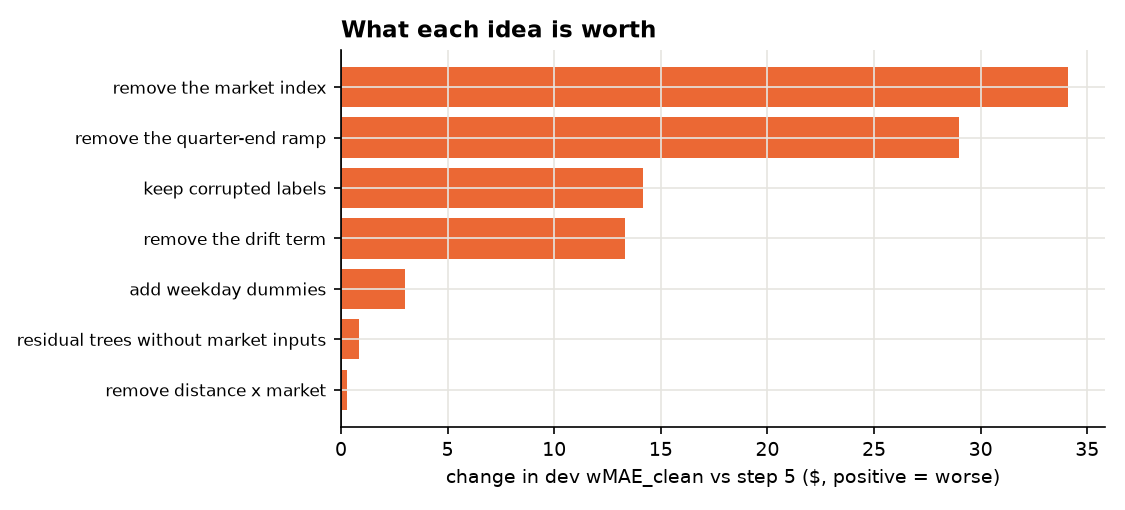
\includegraphics[width=0.8\linewidth]{ablations.png}
  \caption{The same ablations as a chart.}
\end{figure}

\section{Improvement journey}

The final model came out of a sequence of experiments. Each step changed one idea, motivated by what the previous
step got wrong. All six steps were re-run on the same five development folds for this report
(Table~\ref{tab:ladder}, Figure~\ref{fig:ladder}).

\begin{enumerate}
  \item \textbf{Equipment rate per mile $\times$ distance} (\usd{\DevStepA}). The simplest sensible price. It knows
        nothing about place, weight or time.
  \item \textbf{CatBoost on raw dollars} (\usd{\DevStepB}). The original submission. It learns place and weight but
        fits dollars with a squared loss, so the corrupted labels pull it around, and its month features never saw a
        December.
  \item \textbf{LightGBM on log rate with the label screen, market and calendar} (\usd{\DevStepC}). Working on the
        log scale and dropping corrupted labels fix step 2's two worst problems. But trees cannot extend a trend or a
        market level beyond what they saw, so errors stay large when the level moves.
  \item \textbf{Structural ridge} (\usd{\DevStepD}). Time and market enter as straight lines on the log scale, so
        they extrapolate. This step removes most of the remaining error.
  \item \textbf{Ridge plus residual trees} (\usd{\DevStepE}). A small LightGBM learns the local patterns the ridge
        misses, such as a lane's geography interacting with distance and weight.
  \item \textbf{Tuned and recency-weighted} (\usd{\DevStepF}). Tuned spline knots and a larger, slower tree stage
        (Section~\ref{sec:tuning}). Recent loads weigh more, with a time constant of \RecencyTau{} days.
\end{enumerate}

\begin{table}[H]
  \caption{The improvement ladder on the five development folds. ``Change'' is relative to the previous step.}
  \label{tab:ladder}
  \inputtable{ladder}
\end{table}

\begin{figure}[H]
  \centering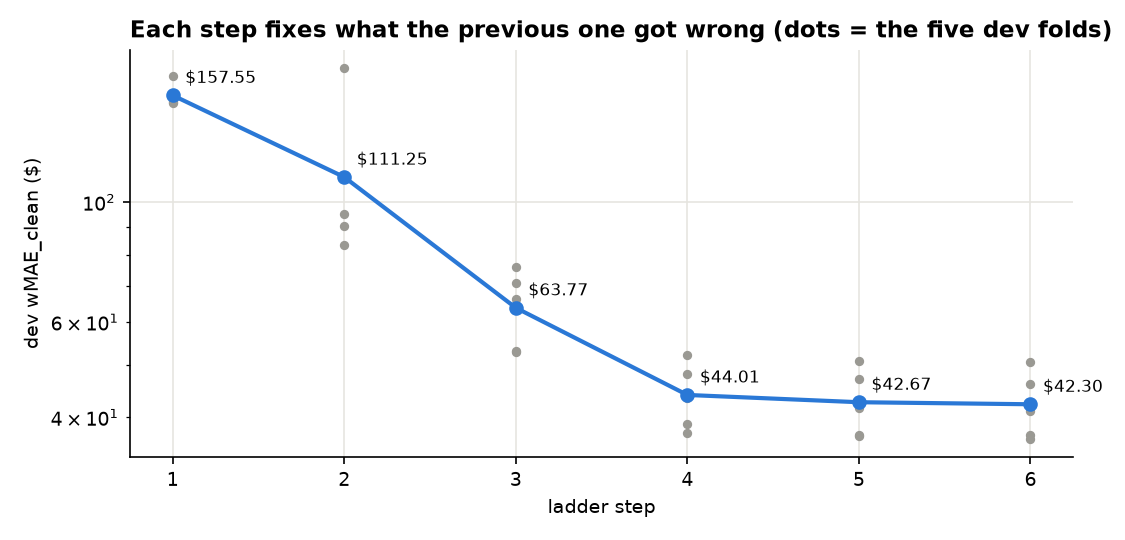
\includegraphics[width=0.85\linewidth]{ladder.png}
  \caption{Development error by ladder step (log scale). Grey dots are the five folds.}\label{fig:ladder}
\end{figure}

Simple time-series baselines sit between steps 2 and 3. The best of them, a cross-section model with the last
daily price level carried forward, scores \usd{\DevNaiveIndex} (Table~\ref{tab:baselines}).

\begin{table}[H]
  \caption{Baselines on the development folds.}\label{tab:baselines}
  \inputtable{baselines}
\end{table}

\begin{table}[H]
  \caption{Paired 7-day block-bootstrap comparisons on the development folds (final minus other model;
  negative means the final model is better).}\label{tab:devci}
  \inputtable{dev_comparisons}
\end{table}

\section{Tuning}\label{sec:tuning}

\textbf{Search.} Optuna \citep{akiba2019optuna} ran \TuneTrials{} trials of its tree-structured Parzen estimator
(seed 42), each scored as the mean development wMAE over the five folds. The locked test was never used. The search
covered the ridge penalty (0.001--10), spline knots (distance 5--12, coordinates 4--9, weight 4--7), the tree
stage (50--600 trees, learning rate 0.01--0.15, 7--63 leaves, 20--300 loads per leaf, L2 penalty 0.001--30,
50--100\% of columns per tree) and recency weighting (off, or a time constant of 45--720 days).

\textbf{Result.} The best trial scores \usd{\TuneBest}; the untuned model scores \usd{\DevStepE}. The best trial is
the configuration frozen in \texttt{configs/final.yaml} (re-found: \TuneMatchesFinal). Table~\ref{tab:tuned} lists
it. The tree stage's size and learning rate matter most (Table~\ref{tab:importance}).

\begin{table}[H]
  \centering
  \begin{minipage}[t]{0.55\linewidth}\centering
    \captionof{table}{Tuned settings.}\label{tab:tuned}
    \small\begin{tabular}{lr}
\toprule
Setting & Tuned value \\
\midrule
Ridge penalty alpha & 0.265 \\
Spline knots: distance / weight / coordinates & 5 / 7 / 4 \\
Recency time constant (days) & 122.6 \\
Residual trees & 293 \\
Learning rate & 0.0215 \\
Leaves per tree & 62 \\
Minimum loads per leaf & 90 \\
L2 penalty lambda & 3.26 \\
Share of columns per tree & 0.81 \\
\bottomrule
\end{tabular}

  \end{minipage}\hfill
  \begin{minipage}[t]{0.4\linewidth}\centering
    \captionof{table}{Most important settings.}\label{tab:importance}
    \small\begin{tabular}{lr}
\toprule
Hyperparameter & Importance (fANOVA) \\
\midrule
n estimators & 0.43 \\
dist knots & 0.12 \\
reg lambda & 0.09 \\
learning rate & 0.09 \\
min child samples & 0.08 \\
\bottomrule
\end{tabular}

  \end{minipage}
\end{table}

\begin{figure}[H]
  \centering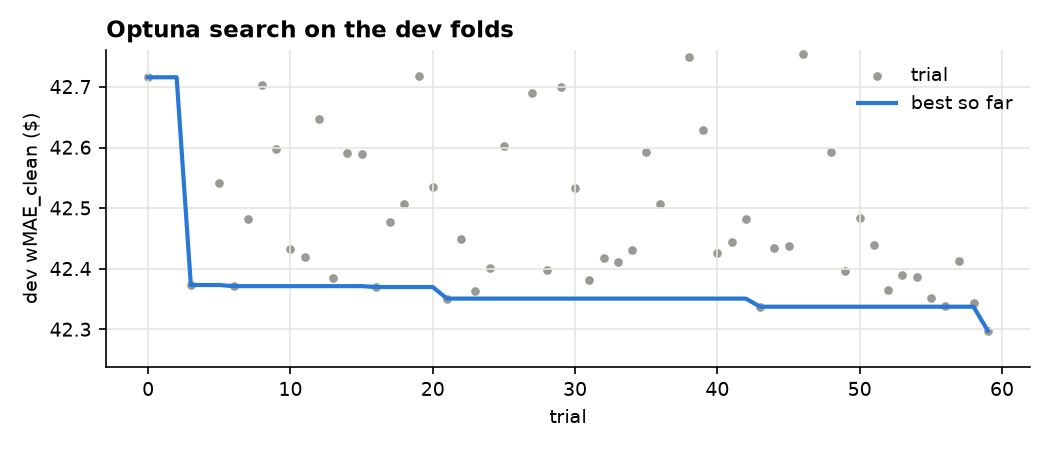
\includegraphics[width=0.75\linewidth]{tuning.png}
  \caption{Trial scores and the best score so far.}
\end{figure}

\textbf{Is the gain real?} Tuning and scoring on the same folds flatters the tuned model. To check, we re-tuned on
folds 1 to $k-1$ only and scored fold $k$ (Table~\ref{tab:nested}). The gains on these unseen folds,
\usd{\NestedGainFour} and \usd{\NestedGainFive}, are close to the in-sample gain of \usd{\DevTunedGain}.

\begin{table}[H]
  \caption{Forward-nested check: tune on earlier folds, score the next one.}\label{tab:nested}
  \inputtable{nested}
\end{table}

\textbf{Honest note.} On the locked test the untuned model was slightly better (Section~\ref{sec:evaluation}). Tuned
and default settings differ by about \TunedDefaultTestPct\% on the test, and by similar amounts in the other
direction on the development folds. They are practically
equivalent. We kept the tuned model because the selection rule was fixed before the test was opened.

\section{Final evaluation}\label{sec:evaluation}

\textbf{Locked test.} Table~\ref{tab:locked} shows every model on September and October 2025, scored once. The
final model's wMAE is \usd{\TestFinalTuned} (\MapeTestFinal\% of the rate). The original CatBoost submission scores
\usd{\TestCatboostRawDollars}; its error is \usd{\TestGapCatboostRawDollars} higher (95\% interval
\TestGapCatboostRawDollarsLow{} to \TestGapCatboostRawDollarsHigh). The untuned step-5 model scores
\usd{\TestRidgePlusResidualTrees}: a difference of $\TestGapRidgePlusResidualTrees$ dollars (interval
$\TestGapRidgePlusResidualTreesLow$ to $\TestGapRidgePlusResidualTreesHigh$), slightly in its favour.

\begin{table}[H]
  \caption{Locked test, September--October 2025. ``vs final'' is the other model's clean MAE minus the final
  model's, with a 95\% paired block-bootstrap interval. Bias is the median log error.}\label{tab:locked}
  \inputtable{locked_test}
\end{table}

\textbf{Including corrupted labels.} On all rows the final model's MAE is \usd{\TestFinalAllMAE}. The difference
from the clean figure is almost entirely the corrupted labels, which no model can predict.

\textbf{Segments.} Errors are similar across equipment types and for new versus known cities, and they grow
with the forecast horizon (Table~\ref{tab:segments}).

\begin{table}[H]
  \caption{Final model on the locked test by segment (clean rows).}\label{tab:segments}
  \inputtable{segments}
\end{table}

\textbf{Residuals.} Figure~\ref{fig:residuals} shows the remaining error. From early October, actual prices sit
about \OctoberUnderForecast\% above the forecast (median, October). Daily errors are strongly autocorrelated, which means a level shift that no available
input explains.

\begin{figure}[H]
  \centering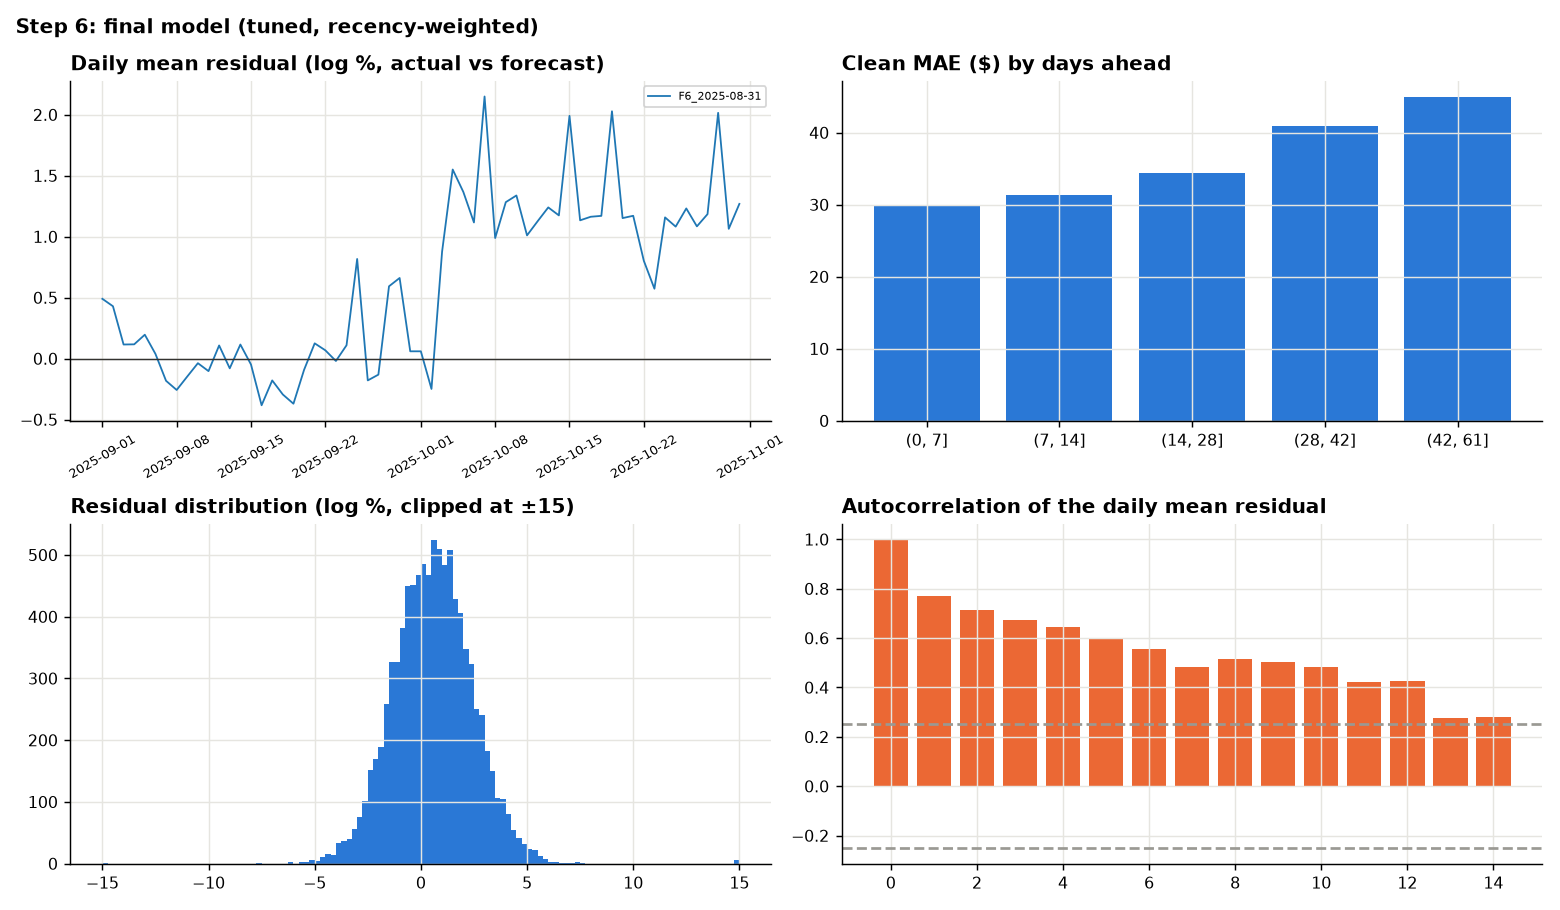
\includegraphics[width=0.95\linewidth]{residuals_test.png}
  \caption{Final model on the locked test: daily mean residual, error by horizon, residual distribution and the
  autocorrelation of daily residuals.}\label{fig:residuals}
\end{figure}

\textbf{Prediction intervals.} We take the 10th/90th and 2.5th/97.5th percentiles of the out-of-sample log errors on
the development folds, per equipment type. On the locked test the 80\% interval covers \CoverEighty\% and the 95\%
interval \CoverNinetyFive\% of clean loads (\CoverEightyAll\% and \CoverNinetyFiveAll\% of all loads). The
intervals are slightly conservative.

\section{December forecast}

The chart rows have no market index and no coordinates. We look the coordinates up from the city list, and take
each day's market index as the mean over that day's loads in \texttt{validation.csv}.

The forecast runs from \usd{\DecMin} to \usd{\DecMax} and ends at \usd{\DecLast} on December 31
(Figure~\ref{fig:december}). The weekly wave follows the market index. The slow rise is the drift plus the
quarter-end ramp.

\begin{figure}[H]
  \centering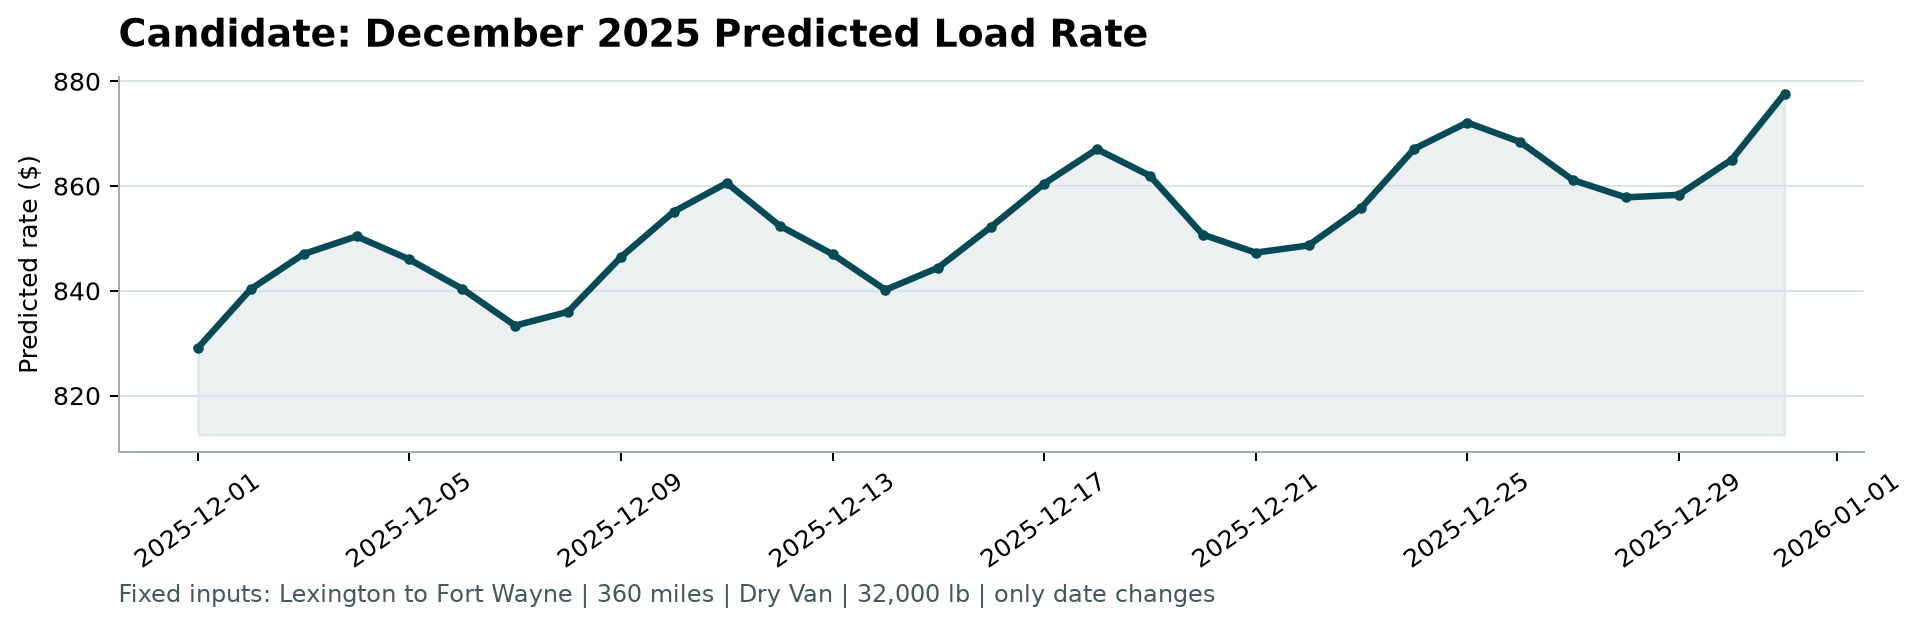
\includegraphics[width=0.95\linewidth]{candidate_december.png}
  \caption{The December chart produced by the assessment's own \texttt{score.py}.}\label{fig:december}
\end{figure}

\textbf{How much rests on the quarter-end ramp?} December has never been observed. The ramp was seen in March, June
and September, and the model assumes it recurs. Without it, December 31 would be \usd{\DecLastNoRamp} instead of
\usd{\DecLast}. If the December market index were unknown and held at its October mean, the line would be a smooth
\usd{\DecFlatMin} to \usd{\DecFlatMax} (Figure~\ref{fig:sensitivity}).

\begin{figure}[H]
  \centering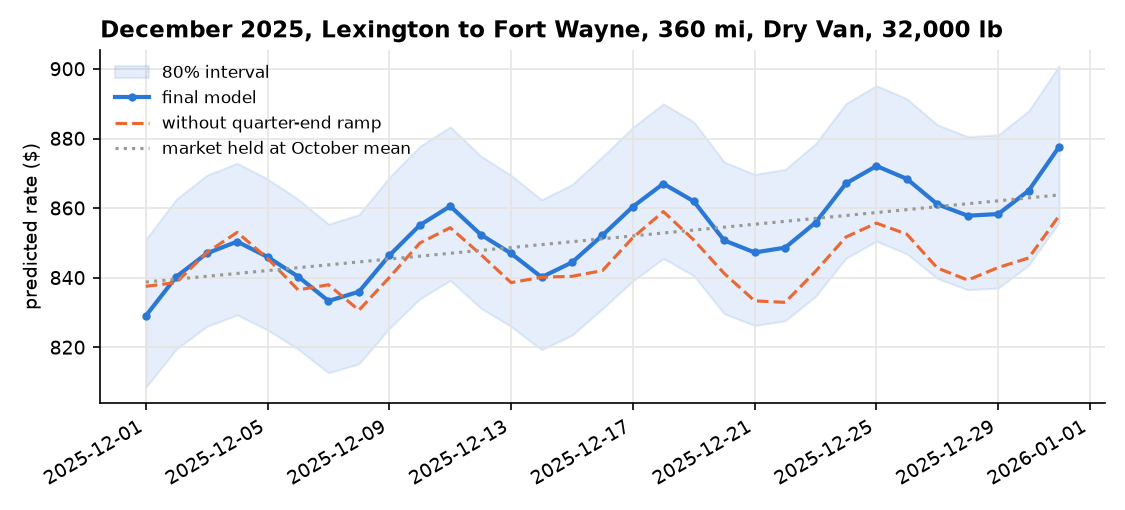
\includegraphics[width=0.9\linewidth]{december_sensitivity.png}
  \caption{December forecast with its 80\% interval, without the quarter-end ramp, and with the market held at its
  October mean.}\label{fig:sensitivity}
\end{figure}

\section{Limitations}

\begin{itemize}
  \item \textbf{Test contamination.} Earlier analyses had already looked at September and October, and the
        quarter-end feature was confirmed there. The locked-test numbers are therefore mildly optimistic.
  \item \textbf{December is an extrapolation.} The labels contain no December. The forecast assumes the
        quarter-end ramp recurs, and holiday effects cannot be learned.
  \item \textbf{Level shifts.} The model cannot anticipate a sudden change in the price level that the market index
        does not show, like the step in early October. In October the actual level sat
        \OctoberUnderForecast\% above the forecast.
  \item \textbf{Market index dependence.} The market index is the most important input. Without the target day's
        index, accuracy falls towards the no-market models (\usd{\AblNoMarket} worse on the development folds).
  \item \textbf{Label noise in scoring.} If the hidden labels contain the same \CorruptPct\% of errors, the all-row
        error will stay near \usd{\TestFinalAllMAE} whatever the model.
  \item \textbf{Synthetic-looking data.} City coordinates are shifted and the data look simulated. Statements about
        freight markets describe this dataset only.
  \item \textbf{Out-of-range geography.} Laredo lies \LaredoDegreesSouth{} degrees of latitude south of every training city, so its
        prices extend the coordinate curves beyond the data.
\end{itemize}

\section{Reproducibility}

Everything runs in Docker. You need Docker with Compose v2, \texttt{make}, and the four CSV files in
\texttt{data/}.

\begin{verbatim}
cp .env.example .env        # choose a database password
make all                    # about 15 minutes on 2 CPU cores
\end{verbatim}

\texttt{make all} runs, in order: \texttt{up} (PostgreSQL 16 and an MLflow 3.5 server with persistent volumes),
\texttt{data-check} (schema and SHA-256 of the inputs), \texttt{experiments} (baselines, the six ladder steps and
seven ablations), \texttt{tune} (\TuneTrials{} Optuna trials and the nested check), \texttt{test-lock} (the
one-shot locked test), \texttt{train} (final fit, export to \texttt{model/}, registration as
\texttt{freight-rate-model@champion}), \texttt{predict} (submission files checked by \texttt{score.py}),
\texttt{report} (this PDF), \texttt{test} and \texttt{lint}.

Every run compares its result with the value logged by the earlier project and stops if they differ by more than
five cents. Seeds are fixed: LightGBM 42, Optuna 42, bootstrap 7, hidden cities 100 plus the fold number. Each
MLflow run records the dataset hashes, git commit, configuration file, parameters, fold manifests, per-fold and mean
metrics, out-of-fold predictions and a residual plot. The MLflow interface is at \texttt{http://localhost:5050}.

The champion training run is \texttt{\ChampionRun} and the locked-test run of the final model is
\texttt{\LockedTestRun}. Fitting takes \FitSeconds{} seconds on all \RowsAfterScreen{} screened loads, and
inference takes about \InferenceMicroseconds{} microseconds per load.


\bibliographystyle{plainnat}
\bibliography{references}

\appendix
\section{Final model parameters}

\begin{table}[H]
  \caption{Resolved parameters of the registered champion (from \texttt{model/final\_params.json}).}
  \inputtable{final_params}
\end{table}

\begin{table}[H]
  \caption{Ridge coefficients of the non-spline terms (log-rate change per unit; the trend is per 100 days).}
  \inputtable{ridge_coefficients}
\end{table}

\section{MLflow run inventory}

\begin{table}[H]
  \caption{Every top-level run behind this report (Optuna trials are nested under \texttt{optuna-search}).}
  \inputtable{run_ids}
\end{table}

\end{document}
